\chapter{Programming of the TransistorTester}
\section{Configuring the TransistorTester}
\label{sec:config}
The complete software for the TransistorTester is available in source code.
The compilation of modules is controlled with a Makefile. The developement was done
at the Ubuntu Linux operating system with the GNU toolchain (gcc version 4.5.3).
It should be possible to use other Linux operating systems without problems.
To load the compiled data to the flash memory or
the EEprom memory, the tool \lcmd{avrdude} (version 6.3) was taken by the Makefile, if you call \inquotes{make upload}.
The program \lcmd{avrdude} \cite{avrdude} is available for Linux and Windows operating system.
The gnu C-compiler gcc is also taken by the AVR studio software and
by the WinAVR \cite{winavr1},\cite{winavr2} software at the Windows operating system.
You can load the program data (.hex and .eep) also with other tools to the ATmega,
but only my Makefile version takes care to load the correct data to the choosed processor.
Avrdude loads only data to the ATmega if the Signature Bytes of the connected ATmega is
identical to the choosed one. 
If you alter the Makefile, all the software will be compiled new, if you call a \lcmd{make} or
\lcmd{make upload} command. The software compiled for a ATmega8 does not run on a ATmega168.
The software compiled for a ATmega328 does not run on the ATmega168! 
A exeption from this rule is the software compiled for ATmega168, this data can also be used
for a ATmega328 without changes.
Be careful, if you don't use my Makefile.

With the correct options set, my software runs on the unchanged hardware of Markus F.
You must set the option PARTNO=M8, \textbf{NOT} the option NO\_AREF\_CAP and \textbf{NOT} the PULLUP\_DISABLE option.
The clock rate can also be set to \(8MHz\) with fuses, no crystal is required!


The following options in the Makefile are avaiable to configure the software for your Tester.

\begin{description} \setlength{\itemsep}{0em}
  \item[PARTNO] describes the target processor:\\
         m8 = ATmega8\\
         m168 or m168p = ATmega168\\
         m328 or m328p = ATmega328\\
         m644 or m644p = ATmega644\\
         m1284p        = ATmega1284\\
         m1280         = ATmega1280\\
         m2560         = ATmega2560\\
    Example:  PARTNO = m168
   \item[UI\_LANGUAGE] specifies the favored Language\\
    LANG\_BRASIL, LANG\_CZECH, LANG\_DANISH, LANG\_DUTCH, LANG\_ENGLISH, \\
    LANG\_GERMAN, LANG\_HUNGARIAN, LANG\_ITALIAN, LANG\_LITHUANIAN, \\
    LANG\_POLISH, LANG\_RUSSIAN, LANG\_SLOVAK, LANG\_SLOVENE, \\
    LANG\_SPANISH  and LANG\_UKRAINIAN is currently avaiable.
 The russian or ukrainian language requires a LCD with cyrillic character set.\\
    Example:  UI\_LANGUAGE = LANG\_ENGLISH

  \item[LCD\_CYRILLIC] is only needed for a LCD-display with cyrillic character set. The \(\mu\) and \(\Omega\) character
is not avaiable with the cyrillic character set.
If you specify this option, both characters are loaded to the LCD with software.
You should set this option, if your display shows wrong characters instead of \(\mu\) or \(\Omega\).\\
Example: CFLAGS += -DLCD\_CYRILLIC

 \item[LCD\_DOGM] must be set, if a LCD with ST7036 controller (Type DOG-M) is used for displaying.
The LCD-contrast is then set with software commands.
If you have changed the contrast value to a wrong value, so that you can not read anything at your display,
you shouls first try to read somthing from a side look to the display.
If this fails also, you should reset the EEprom to the initial values with a ISP programmer.\\
Example: CFLAGS += -DLCD\_DOGM

 \item[FOUR\_LINE\_LCD] can be used with a 4x20 character display for better using the additional space.
Additional parameters, which are shown only short in row 2, will be shown in row 3 and 4 with this option.
With graphic displays, the number of lines is determined from the display height and the line spacing.\\
Example: CFLAGS += -DFOUR\_LINE\_LCD

  \item[LCD\_LINE\_LENGTH] specifies the number of characters that can be displayed in one line. 
With graphic displays, the number of characters is calculated from the character width and the display width.\\
Example: CFLAGS += -DLCD\_LINE\_LENGTH=20

  \item[DD\_RAM\_OFFSET] Somne character displays use different DD-RAN starting addresses for the beginning of each line.
Usually the DD-RAM starting address for line 1 is 0.
Some displays like TC1604 or TC1602 use a 128 (0x80) for the beginning of line 1.
This can be respected with this option.
Example: CFLAGS += -DDD\_RAM\_OFFSET = 128

  \item[WITH\_LCD\_ST7565] This option must be used, if a 128x64 pixel LCD is connected with serial
interface. For this display type further options must be set, which are described in table~\ref{tab:cod-display}.
You can also use the simular SSD1306 controller instead of the ST7565 controller for example.
This must be done by setting the variable WITH\_LCD\_ST7565 to 1306.
A PCF8812 or PCF8814 Controller is also supported, if the Option is set correctly.
Also a display with a ST7920 or NT7108 controller can be connected.
For the NT7108 controller a additional serial-parallel converter 74HC(T)164 or 74HC(T)595 must be used.  \\
Example: WITH\_LCD\_ST7565 = 1 

 \item[LCD\_INTERFACE\_MODE] For the SSD1306 controller also the I\textsuperscript{2}C type interface with address 0x3c
can be used  instead of the 4-wire SPI interface by setting this option to 2.
For the ST7920 controller a special serial interface can be selected by setting this option to 5.
If only one connection type is provided for a controller, you need not set the constant LCD\_INTERFACE\_MODE .
All currently used values for LCD\_INTERFACE\_MODE and WITH\_LCD\_ST7565 are shown in table~\ref{tab:cod-display}. \\

\begin{table}[H]
  \begin{center}
    \begin{tabular}{| c | c | c | c|}
    \hline
 Display-Type       &  Interface       & WITH\_LCD\_ST7565 &  LCD\_INTERFACE\_MODE \\
    \hline
    \hline
  Character 16x2,   & 4-Bit parallel   &  disabled (0)     & disabled (1) \\
  Character 20x4    &  4-Wire SPI       &                   &    4   \\
                  & I\textsuperscript{2}C &                &   2    \\
    \hline
  Graphic ST7565    & 4-Wire SPI        &   1 or 7565       &  disabled (4) \\
    \hline
  Graphic ST7565  & I\textsuperscript{2}C & 1 or 7565      &   2 \\
    \hline
  Graphic SSD1306   & 4-Wire SPI        &   1306            &  disabled (4) \\
    \hline
  Graphic SSD1306  & I\textsuperscript{2}C & 1306          &   2 \\
    \hline
  Graphic ST7920    & 4-Bit parallel   &   7920            &  disabled (1) \\
    \hline
  Graphic ST7920    & 2-Bit serial     &   7920            &  5 \\
    \hline
  Graphic NT7108    & 8-Bit parallel   &   7108            &  disabled (6) \\
    or KS0108       &    + 74HCT164    &                   &      \\
    \hline
  Graphic PCF8812   & 4-Wire SPI       &   8812            & disabled (4) \\
    \hline
  Graphic PCF8814   & 4-Wire SPI       &   8814            & disabled (4) \\
                  & I\textsuperscript{2}C & 8814           &   2 \\
                    & 3-line           &   8814            &   3 \\
    \hline
  Graphic ILI9163   & 4-Wire SPI       & 9163              & disabled (4) \\
  128x128 Color     &                 &                   &              \\
    \hline
  Graphic ST7735    & 4-Wire SPI       & 7735              & disabled (4) \\
  128x160 Color     &                 &                   &              \\
    \hline
    \end{tabular}
  \end{center}
  \caption{Number setting for controller and interface mode}
  \label{tab:cod-display}
\end{table}

The values in brackets are used software internal and are shown for information only.
You should not set the values in brackets here in the Makefile.\\

Example: CFLAGS += -DLCD\_INTERFACE\_MODE=2

  \item[LCD\_SPI\_OPEN\_COL] With the option LCD\_SPI\_OPEN\_COL the data signals of the SPI interface
are not switched to VCC directly.
The signals are switched to GND only, for high signals the pullup resistors of the ATmega are used.
For the RESET signal a external pull-up resistor is required, if the option PULLUP\_DISABLE is set.
For the other signals the internal pullup resistors of the ATmega are temporary used,
even if option PULLUP\_DISABLE is set.
Example: CFLAG += -DLCD\_SPI\_OPEN\_COL

\item[LCD\_I2C\_ADDR] The I\textsuperscript{2}C address of the SSD1306 controller can be selected to 0x3d by presetting
the constant LCD\_I2C\_ADDR to 0x3d.\\
Example: CFLAGS += -DLCD\_I2C\_ADDR=0x3d

  \item[LCD\_ST7565\_RESISTOR\_RATIO] With this option the resistor ratio for the voltage regulator of
the ST7565 controller is set.
Usually values between 4 and 7 are practical.
The value can be set between 0 and 7.\\
Example: LCD\_ST7564\_RESISTOR\_RATIO = 4

  \item[LCD\_ST7565\_H\_FLIP] With this option the display content can be flipped in horizontal direction.\\
Example: CFLAGS += -DLCD\_ST7565\_H\_FLIP = 1

  \item[LCD\_ST7565\_H\_OFFSET] This option can be used to adapt the display window to the used memory area.
 The controller uses more horizontal pixel (132) as the display window shows (128).
 Depending of your display module a value of 0, 2 or 4 can be required for proper presentation.\\
Example: CFLAGS += -DLCD\_ST7565\_H\_OFFSET = 4

  \item[LCD\_ST7565\_V\_FLIP] With this option the display content can be flipped in vertical direction.\\
Example: CFLAGS += -DLCD\_ST7565\_V\_FLIP = 1

  \item[VOLUME\_VALUE] You can predefine a contrast value for ST7565 or SSD1306 controllers.
The value for the ST7565 controller can be between 0 and 63. For the SSD1306 controller you can
select a value between 0 and 255.\\
Example: CFLAGS += -DVOLUME\_VALUE = 25

  \item[LCD\_ST7565\_Y\_START] With this option you can set the first row correctly to the top of screen.
The first row is shifted to the middle of the screen for some display variants.
For this variants you can shift the first row to the top of the screen again,
if this option is set to 32 (half of the screen height).\\
Example: CFLAGS += -DLCD\_ST7565\_Y\_START = 32

  \item[LCD\_CHANGE\_COLOR] This option expand the menu functions with a selection item
to change the background and the foreground color.
If the value is set to 2, the colors blue and red are swapped.
You can select this option only for color displays (controller ST7735 or ILI9163).\\
Example: CFLAGS += -DLCD\_CHANGE\_COLOR=1

 \item[LCD\_BG\_COLOR] With this 16-bit value you can select a background color.
Normally the upper 5 bits are used for the color red, the middle 6 bits are used for the color green
and the lower 5 bits are used for the color blue. Sometimes the bits for the colors red and blue
are swapped.
You can select this option only for color displays (controller ST7735 or ILI9163).\\
Example: CFLAGS += -DLCD\_BG\_COLOR=0x000f

 \item[LCD\_FG\_COLOR] With this 16-bit value you can select a forground color.
The example selects the color white for text and symbols.
You can select this option only for color displays (controller ST7735 or ILI9163).\\
Example: CFLAGS += -DLCD\_FG\_COLOR=0xffff

  \item[FONT\_8X16] You must select one font size for the ST7565 controller.
Selectable are different fonts with the name \inquotes{FONT\_} with appended size information (width X height).
Currently the font sizes 6X8, 8X8, 7X12, 8X12, 8x12thin, 8X14, 8X15, 8X16, and 8X16thin are available.
Font size 8X16 or 8x16thin is the most efficient use of graphics space for a 128x64 pixel LCD.\\
Example: FONT\_8X16

 \item[BIG\_TP] The pin numbers for the graphical presentation can be shown bigger with this option.\\
Example: CFLAGS += BIG\_TP

 \item[INVERSE\_TP] With this option you can select a inverse presentation (white background) of the pin numbers
on the graphical display.
Because a boarder in required for this presentation, you can not combine this option with the BIG\_TP option.\\
Example: CFLAGS += INVERSE\_TP

  \item[STRIP\_GRID\_BOARD] This option adapts the software to a changed port D connection for strip grid printed boards.
You can find the details in the chapter hardware~\ref{sec:hardware} at page~\pageref{sec:hardware}.
You can also choose alternative assignments of ATmega pins for graphical displays.
For the chinese \inquotes{T5} board you must set the STRIP\_GRID\_BOARD option to 5.
For alternative pin assignments of graphical displays the assignment of the pushbutton signal is unchanged.\\
Example: CFLAGS += -DSTRIP\_GRID\_BOARD

  \item[WITH\_MENU] activated a menu function for a ATmega328. You can select some additional functions with a
selection menu, which you can call with a long key press (\textgreater~0.5s).\\
Example: CFLAGS += -DWITH\_MENU

 \item[MAX\_MENU\_LINES]
This option specifies a maximum count of lines for the shown choices of menu items.
Normally the count of lines for the menu items is given by the present count of lines of the display.
Because there are usually more items selectable as the display can support,
the choices are replaced in a cyclic manner.
Building the display content in this cyclic way will take several time, especially for big color displays 
with many lines.
With the limitation of the line count by this option you can reduce the output time for the menu choices significant,
which will speed up the operation.
The default value for this item is 5.\\
Beispiel: CFLAGS += -DMAX\_MENU\_LINES=3


  \item[WITH\_ROTARY\_SWITCH] The menu function can be easier controlled with a the extension of a rotary pulse encoder.
See the description~\ref{fig:RotExt} in the Hardware section for details of the required extension.
If your rotary pulse encoder has the same count of indexed positions (detent) as pulses of the switch for every turn, you must
set the  option WITH\_ROTARY\_SWITCH to 2. If the rotary pulse encoder has twice the count of indexed position, you must
set the option WITH\_ROTARY\_SWITCH to 1.
Setting the WITH\_ROTARY\_SWITCH to 5 selects the highest resolution for the rotary switch. Every cycle of the two switches results
to a count of 4. Usually this setting is only usefull for rotary switch encoders without indexed positions.
A setting of the WITH\_ROTARY\_SWITCH to 4 is required for correct handling of two separate push buttons for Up and Down,
which are installed instead of the normal rotary encoder switches.
Do not use a setting of 4 for normal rotary encoders!\\
Example: CFLAGS += -DWITH\_ROTARY\_SWITCH=1

  \item[CHANGE\_ROTARY\_DIRECTION] You can change the direction of the detected rotary direction by hardware swap of
the two switch signals or by setting the this option.\\
Example: CFLAGS += -DCHANGE\_ROTARY\_DIRECTION

  \item[WITH\_SELFTEST] If you specify this Option, software will include a selftest function.
Selftest will be started, if you connect all three probes together and start measurement.
If the menu function is selected, only the calibration part of the self test is executed by automatic start with
shorted probes. The selftest parts T1 to T7 are only executed, if the selftest is started with menu selection.\\
Example: CFLAGS += -DWITH\_SELFTEST

  \item[NO\_COMMON\_COLLECTOR\_HFE] disables the hFE measurement of transistors with the common collector circuit.
You can save memory to enable the extended selftests T1 to T7 for a ATmega168 processor.
By default both measurement circuits for the hFE measurement are enabled, 
but there is no place in the program memory of the ATmega168 for the extended selftests.\\
Example: CFLAGS += -DNO\_COMMON\_COLLECTOR\_HFE

  \item[NO\_COMMON\_EMITTER\_HFE] disables the hFE measurement of transistors with the common emitter circuit.
You can save memory to enable the extended selftests T1 to T7 for a ATmega168 processor.
By default both measurement circuits for the hFE measurement are enabled, 
but there is no place in the program memory of the ATmega168 for the extended selftests.\\
Example: CFLAGS += -DNO\_COMMON\_EMITTER\_HFE

  \item[NO\_TEST\_T1\_T7] This option disable the execution of the selftest parts T1 to T7.
This tests are usefull to find errors in the hardware like incorrect measurement resistors or isolation problems.
If your hardware is well, you can omitt this selftest parts T1 to T7 by setting this option to get a faster calibration.
With enabled menu function the selftest parts T1 to T7 are only started by selection of the menu function \inquotes{Selftest}.
The ATmega168 processor does not use the selftest parts T1 to T7, if both measurement types for hFE determination are used.\\
Example: CFLAGS += -DNO\_TEST\_T1\_T7

  \item[AUTO\_CAL] The zero offset for capacity measurement will be written additionally
to the EEprom with the selftest routine. Additionally the offset voltage of the analog comparator (with option REF\_C\_KORR) and the
voltage offset of the internal reference voltage (REF\_R\_KORR) will be measured automatically, if you connect a
capacitor with a capacity value between \(100nF\) and \(20\mu F\) to pin~1 and pin~3 after measurement of capacity zero offset. 
All found values will be written to EEprom and will be used for further measurements automatically.
The port output resistance values will be determined at the beginning of each measurement.\\
Example: CFLAGS += -DAUTO\_CAL

  \item[SHORT\_UNCAL\_MSG] After the test of a part a message is shown for processors with at least 32K flash memory,
if the tester is still uncalibrated. Normally followes after the hint a short description, how the
tester can be calibrated. This description is not shown, if you set the option SHORT\_UNCAL\_MSG in the Makefile.
With this option set, the tester only display a one line hint.
This reduces the required space of flash memory  and also the display time for the user,
which already know, how to calibrate the tester.\\
Example: CFLAGS += -DSHORT\_UNCAL\_MSG

 \item[NO\_ICONS\_DEMO]
This option will switch off the additional demonstration of the icons and the output of the character set with
the menu function \inquotes{Show data}.
This reduces the required space of flash memory  and also the display time for the user.\\
Example: CFLAGS += -DNO\_ICONS\_DEMO

 \item[WITH\_ROTARY\_CHECK]
This option enables the additional menu function for the test of a rotary encoder.
For the test you must connect a rotary encoder to the test pins TP1, TP2 and TP3.
Please note, that you can not check the build-in rotary-encoder of the tester!
You can also use a rotary encoder for ease in operation of the tester with the option WITH\_ROTARY\_SWITCH.\\
Example: CFLAGS += -DWITH\_ROTARY\_CHECK

 \item[NO\_FREQ\_COUNTER]
With this option you can deselect the frequency counter function of the tester.
This is especially useful if the pin PD4 (ATmega328) can not be used together with the
connected display.
The corresponding entry in the list of menu functions then no longer appears and also
Flash memory space is saved.\\
Example: CFLAGS += -DNO\_FREQ\_COUNTER

 \item[WITH\_FREQUENCY\_DIVIDER]
With this option the menu is expanded by a selectable prescaler for the frequency counter.
The scaler can be selected to 1:1, 1:2, 1:4, 1:8, 1:16, 1:32, 1:64 and 1:128 .
This option is only useful, if a external prescaler can be connected to the frequency input of the tester.
The shown frequencies and periodes of the measurements will respect the selected scaling factor.\\
Example: CFLAGS += -DWITH\_FREQUENCY\_DIVIDER

 \item[NO\_FREQUENCY\_SWITCH]
With this switch you can deselect the support of the frequency input switch of the ATmega644/ATmega1284 circuit.
The support of the LF and HF crystal measurement will not be supported with this option.\\
Example: CFLAGS += -DNO\_FREQUENCY\_SWITCH=1

\item[PWM\_SERVO] 
will select a special PWM generation for testing servos instead of a general purpose PWM generation.\\
Example: CFLAGS += -DPWM\_SERVO=1

  \item[WITH\_SamplingADC] With this option set, the tester make use of the sampling method of ADC in special cases.
By shifting the sampling time of the ADC with increments of 1, 4 or 16 processor clock intervals for repeatable signals
fast changes of voltages can be monitored.
The load time of little capacitors below \(100pF\) can be monitored with a resulting resolution of \(0.01pF\) with a \(16MHz\) processor clock.
With the same method the resonant frequency of little coils below \(2mH\) can be monitored with a parallel capacitor to build a LC-resonator.
If the capacity of the parallel capacitor is known, the inductance of the coil can be calculated with high resolution from
the resonant frequency. As a side product the quality factor Q can be estimated from the resonant behavior.
This features are switched on by setting the option WITH\_SamplingADC.
At the calibration sequence additionally the zero capacity values of the sampling method is measured and
after that the capacity value of a suitable capacitor for later building the LC-resonator with a unknown coil is measured.\\
Example: WITH\_SamplingADC = 1

  \item[WITH\_XTAL]
This option enables additional tests for crystals and resonators, if the SamplingADC function is also enabled and
a 16~MHz crystal is used for clock generation (OP\_MHZ = 16).
If possible, the frequencies for serial and parallel circuit is measured and than the serial capacity Cm of the
equivalent circuit is tried to compute from the frequency offset.\\
Example: CFLAGS += -DWITH\_XTAL

  \item[WITH\_UJT]
This option enables additional tests for  Unijunction transistors. 
If the SamplingADC function is enabled, the tester tries to build a oscillator with the part.
But the UJT type is also detected without the SamplingADC function.
Without the option WITH\_UJT the unijunction transistors are detectes as double diode.\\
Example: CFLAGS += -DWITH\_UJT

  \item[WITH\_PUT]
This option enables a additional test for \inquotes{Programmable Unijunction Transistor}.
Without this option PUTs are usually detected as Bipolar Junction Transistor.\\
Example: CFLAGS += -DWITH\_PUT

 \item[FET\_Idss]
This option enables additional measurements to compute the drain current Idss, if the estimation is not
above \(60mA\). The estimation and calculation is done with a assumed quadratical current propagation.\\
Example: CFLAGS += -DFET\_Idss

  \item[FREQUENCY\_50HZ] At the end of selftest a 50~Hz Signal will be generated on Port~2 and Port~3 for up to one minute.
 This option should be set only for special cases to check the delay function.\\
Example: CFLAGS += -DFREQUENCY\_50HZ

  \item[CAP\_EMPTY\_LEVEL]  This option defines the voltage level for discharged capacitor (mV units).
You can set the level to higher value as \(3mV\), if the tester does not finish discharging of capacitors.
In this case the tester ends after longer time with the message \inquotes{Cell!}.\\
Example: CFLAGS += -DCAP\_EMPTY\_LEVEL=3

  \item[WITH\_AUTO\_REF] specifies, that reference voltage is read to get the actual factor for capacity measuring of low capacity values (below \(40\mu F\)).\\
Example:  CFLAGS += -DWITH\_AUTO\_REF

  \item[REF\_C\_KORR] specifies a offset for readed reference voltage in mV units.
This can be used to adjust the capacity measurement of little capacitors.
A correction value of 10 results to about 1~percent lower measurement results.
If the option AUTO\_CAL is selected together with the WITH\_SELFTEST option, the REF\_C\_KORR will be
a offset to the measured voltage difference of the test capacitor and the internal reference voltage.\\
Example:  CFLAGS += -DREF\_C\_KORR=14

  \item[REF\_L\_KORR] specifies a additional offset in mV units to the reference voltage for the measurement of
inductance values. 
The REF\_C\_KORR offset and respectively the offset value from the calibration is additionally used with the inductance measurement.
The REF\_L\_KORR value will be subtracted for measurements without a \(680\Omega\) resistor,
for measurements with a \(680\Omega\) resistor the value will be added.
A correction value of 10 will change the result about 1 percent.\\
Example: CFLAGS += -DREF\_L\_KORR=40

  \item[C\_H\_KORR] specifies a correction value for the measurement of big capacitor values.
A value of 10 results to 1~percent lower measurement results.\\
Example:  CFLAGS += -DC\_H\_KORR=10

  \item[WITH\_UART] uses the pin PC3 as output for the serial text (V24).
If the option is not set, the pin PC3 can be used for reading a external voltage with a 10:1 resistor divider.
With this equipment you can check the breakdown voltage of zener diodes, which have more than \(4.5V\) breakdown voltage.
This measurement will repeat with 3 measurements per second until you release the Start button.\\
Example: CFLAGS += -DWITH\_UART

  \item[WITH\_HARDWARE\_SERIAL] is only used to enable serial output for testers build with the Arduino UNO board.\\
Example:  CFLAGS += -DWITH\_HARDWARE\_SERIAL

  \item[TQFP\_ADC6] The Option TQFP\_ADC6 uses the additional input ADC6 of the ATmega with TQFP or QFN package instead of
the PC3 pin (ADC3).
With this option the external voltage input can be used independent of the usage of PC3 pin for serial output.
The ADC6 input is then used for the zener diode measurement and for the dialog selectable external voltage measurement
for a ATmega328.\\
Example: CFLAGS += -DTQFP\_ADC6

  \item[TQFP\_ADC7] The Option TQFP\_ADC7 uses the additional input ADC6 of the ATmega with TQFP or QFN package instead of
the PC3 pin (ADC3).
With this option the external voltage input can be used independent of the usage of PC3 pin for serial output.
If this option is used without the option TQFP\_ADC6, both the zener diode measurement and the measurement of external voltage
with the dialog is done with the ADC7 analog input.
If this option is used together with the TQFP\_ADC6 option, is the zener diode measurement done with the ADC6 pin and
both pins are used for voltage measurement with the dialog of the ATmega328.
Both ADC input pins shouls be assembled with a 10:1 voltage divider.\\
Example: CFLAGS += -DTQFP\_ADC7

  \item[WITH\_VEXT] enables the measurement of a external voltage with a 10:1 voltage divider.
For the ATmega168 or ATmega328 processor usually the PC3 pin is used as input, if no option TQFP\_ADC6 or
TQFP\_ADC7 is set. In this case this option is only possible, if the WITH\_UART option is not set.\\
Example: CFLAGS += -DWITH\_VEXT 

  \item[RMETER\_WITH\_L] select for the resistor measurement function, which is selected with a resistor at TP1 and TP3,
additionally the measurement of inductance. The operation mode is indicated with a \textbf{[RL]} at the end of the first display line.
With the additional test for inductance the measurement time is increased for resistors below \(2100\Omega\) considerably.
Also resistors below \(10\Omega\) will not be measured with the ESR methode Without this option, because
a part with inductance can not be excluded. Because the ESR measurement method  uses short current pulses,
parts with inductance can not be measured. The resistors below \(10\Omega\) can only measured with a resolution of
\(0.1\Omega\) without this option, because only with the ESR method a resolution of \(0.01\Omega\) can be obtained.
If this option is set, the previous limitations are not affected, but the measurement time can be longer.\\
Example: CFLAGS += -DRMETER\_WITH\_L

  \item[AUTOSCALE\_ADC] enables the automatic scale switchover of the ADC to either VCC or internal reference.
Internal reference gives a \(2.56V\) scale for ATmega8 and a \(1.1V\) scale for other processors.
For the ATmega8 the automatic scale switchover is not used any more.\\
Example: CFLAGS += -DAUTOSCALE\_ADC

  \item[ESR\_ZERO] defines a zero offset for ESR measurements.
The zero offsets for all three pin combinations will be determined with the selftest and replaces the preset zero offset.
This zero offsets will be subtracted from all ESR measurements.\\
Example: CFLAGS += -DESR\_ZERO=29

  \item[NO\_AREF\_CAP] tells your Software, that you have no capacitor (\(100nF\)) installed at pin AREF (pin 21).
This enables a shorter wait-time for the AUTOSCALE\_ADC scale switching of the ADC.
A \(1nF\) capacitor was tested in this mode without detected errors.
Figure~\ref{pic:aref1} and \ref{pic:aref5} show the switching time with a \(1nF\) capacitor.
As you can see the switching from \(5V\) to \(1.1V\) is much slower than switching back to \(5V\). If you
have still installed the \(100nF\), switching time will be about factor 100 longer!\\
Example: CFLAGS += -DNO\_AREF\_CAP
\end{description}
\begin{figure}[H]
  \begin{subfigure}[b]{.5\textwidth}
    \centering
    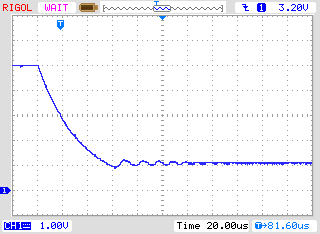
\includegraphics[width=.95\textwidth]{../PNG/AREF2_1V.png}
    \caption{from 5V to 1.1V }
    \label{pic:aref1}
  \end{subfigure}
  ~
  \begin{subfigure}[b]{.5\textwidth}
    \centering
    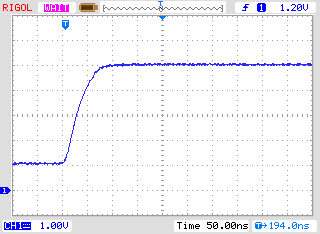
\includegraphics[width=.95\textwidth]{../PNG/AREF2VCC.png}
    \caption{from 1.1V to 5V}
    \label{pic:aref5}
  \end{subfigure}
  \caption{AREF switching with a \(1nF\) Capacitor}
\end{figure}

\begin{description} \setlength{\itemsep}{0em}
  \item[REF\_R\_KORR] specifies a offset for the internal ADC-reference voltage in mV units.
With this offset a difference by switching from VCC based ADC reference to internal ADC reference for resistor measurement can be adjusted.
If you select the AUTO\_CAL option of the selftest section, this value is only a additionally offset to the found voltage 
difference in the AUTO\_CAL function.\\
Example: CFLAGS += -DREF\_R\_KORR=10

  \item[OP\_MHZ] tells your software at which Clock Frequency in MHz your Tester will operate.
The software is tested only for \(1MHz\), \(8MHz\) and additionally \(16MHz\). 
The \(8MHz\) operation is recommended for better resolution of capacity and inductance measurement.\\
Example: OP\_MHZ = 8

  \item[RESTART\_DELAY\_TICS] must be set to 6, if the ATmega168 or ATmega328 is used with the internal RC-oszillator instead of
the crystal oszillator.
If this value is not preset, the software respects the 16384 clock tics delay for restart from sleep mode with the crystal operation.\\
Example: CFLAGS += -DRESTART\_DELAY\_TICS=6

  \item[USE\_EEPROM] specifies if you wish to locate fix text and tables in EEprom Memory. Otherwise the flash memory is used.
Recommended is to use the EEprom (option set).\\
Example: CFLAGS += -DUSE\_EEPROM

\item[EBC\_STYLE] specifies, that the output of transistor pin layout is done with format \inquotes{EBC=...} or \inquotes{GDS=...}.
This way of output save program memory for the ATmega. Without this option the layout is shown with the
format \inquotes{123=...}, where every point represent a E~(Emitter), B~(Base) or C~(Collector).
For FET transistors every point can be a G~(Gate), D~(Drain) or S~(Source).
If the sequence of the test pins is not 1, 2 and 3 in the reading direction, you can invert the sequence with the option
EBC\_STYLE=321 . The pin assignment is then shown with style \inquotes{321=\dots}, which will better match the usual
reading direction, if the testpin sequence is 3,2,1 .\\
Example: CFLAGS += EBC\_STYLE

  \item[NO\_NANO] specifies that the decimal prefix nano will not be used to display the measurement results.
So capacity values will be shown in \(\mu F\) instead of \(nF\).\\
Example: CFLAGS += NO\_NANO

  \item[NO\_LONG\_PINLAYOUT] can be set to prevent the long style of pin layout for graphical displays 
like \inquotes{ Pin  1=E 2=B 3=C}.
If the option is set, the short style is used instead like \inquotes{ Pin  123=EBC}.\\
Example: CFLAGS += NO\_LONG\_PINLAYOUT

\item[PULLUP\_DISABLE] specifies, that you don't need the internal pull-up resistors.
 You must have installed a external pull-up resistor at pin~13 (PD7) to VCC, if you use this option.
This option prevents a possible influence of pull-up resistors at the measuring ports (Port~B and Port~C).\\
Example: CFLAGS += -DPULLUP\_DISABLE

  \item[ANZ\_MESS] this option specifies, how often an ADC value is read and accumulated.
You can select any value between 5 and 200 for building mean value of one ADC measurement.
Higher values result to better accuracy, but  longer measurement time.
One ADC measurement with 44~values takes about \(5ms\).\\
Example: CFLAGS += -DANZ\_MESS=25

  \item[POWER\_OFF] This option enables the automatic power off function. If you don't specify this option,
 measurements are done in a loop infinitely  until power is disconnected with a ON/OFF switch.
If you have the tester without the power off transistors, you can deselect the option POWER\_OFF.

If you have NOT selected the POWER\_OFF option with the transistors installed,
you can also shut down the tester, if you have selected the WITH\_MENU option.

You can also specify, after how many measurements without a founded part the tester will shut down.
The tester will also shut down the power after twice as much measurements are done in sequence without a
single failed part search. If you have forgotten to unconnect a test part, total discharging of battery is avoided. 
Specify the option with a form like CFLAGS += -DPOWER\_OFF=5 for a shut off after 5 consecutive measurements
without part found. Also 10~measurements with any founded part one after another will shut down.
Only if any sequence is interrupted by the other type, measurement continues.
The result of measurement stay on the display for 28~seconds for the single measurement, for the
multiple measurement version display time is reduced to 5~seconds (set in config.h).
If the start key is pressed a longer time on power on time, the display time is also 28~seconds for the multiple measurement.
The maximum value is 255 (CFLAGS += -DPOWER\_OFF=255).\\
Example 1: CFLAGS += -DPOWER\_OFF=5\\
Example 2: CFLAGS += -DPOWER\_OFF

  \item[BAT\_CHECK] enables the Battery Voltage Check. If you don't select this option, the version number of
software is output to the LCD instead.
This option is usefull for battery powered tester version to remember for the battery change.\\
Example: CFLAGS += -DBAT\_CHECK

  \item[BAT\_OUT] enables Battery Voltage Output on LCD (if BAT\_CHECK is selected).
 If your \(9V\) supply has a diode installed, use the BAT\_OUT=600 form to specify the threshold voltage (mV) of your diode
to adjust the output value.
Also the voltage loss of transistor T3 can be respected with this option.
 threshold level does not affect the voltage checking levels (BAT\_POOR).\\
Example 1: CFLAGS += -DBAT\_OUT=300\\
Example 2: CFLAGS += -DBAT\_OUT

  \item[BAT\_POOR] sets the poor level of battery voltage to the specified 1mV value.
The warning level of battery voltage is \(0.8V\) higher than the specified poor level, if the poor level is more than \(5.3V\).
If the poor level is \(5.3V\) or less, the warning level is \(0.4V\) higher. If the poor level is below \(3.25V\), the
warning level is only \(0.2V\) higher than the selected poor level and if the poor level is below \(1.3V\), the
warning level is only \(0.1V\) higher than the specified poor level.
Setting the poor level to low values such as \(5.4V\) is not recommended for rechargeable \(9V\) batteries,
because this increase the risk of battery damage by the reason of the deep discharge!
If you use a rechargeable \(9V\) Battery, it is recommended to use a Ready To Use type, because of the lower self-discharge.\\
Example for low drop regulator (\(5.4V\)): CFLAGS += -DBAT\_POOR=5400\\
Example for 7805 type regulator (\(6.4V\)): CFLAGS += -DBAT\_POOR=6400

  \item[DC\_PWR] This voltage level in mV units specify the battery voltage above which the tester
changes to the \inquotes{DC\_Pwr\_Mode}. Normally the tester operates in a battery mode, where all additional
functions are limited in time. With the \inquotes{DC\_Pwr\_Mode} the tester runs the additional functions with unlimited time.
Because there is no DC-DC converter operating with \(0.9V\) input voltage,
the \inquotes{DC\_Pwr\_Mode} is also entered, if the battery voltage is detected below \(0.9V\). \\
Example: CFLAGS += -DDC\_PWR=9500

 \item[BAT\_NUMERATOR] defines the numerator of a fraction used for scaling the input voltage to get the right
battery voltage.
For a normal voltage divider build with a \(10 k\Omega\) and a \(3.3 k\Omega\) resistor you get a fraction 
of (10000 + 3300)/3300. 
You should reduce the fraction to 133/33 .\\
Example: CFLAGS += -DBAT\_NUMERATOR=133

 \item[BAT\_DENOMINATOR] specifies the denominator of a fraction, which is used to scale the voltage value.\\
Example: CFLAGS += -DBAT\_DENOMINATOR=33

 \item[EXT\_NUMERATOR] defines the numerator of a fraction used for scaling the external input voltage.
 With a voltage divider build with a \(180 k\Omega\) and a \(20 k\Omega\) resistor the fraction is (180000 + 20000)/20000 .
You should reduce the fraction to 10/1 .\\
Example: CFLAGS += -DEXT\_NUMERATOR=10

 \item[EXT\_DENOMINATOR] specifies the denominator for the fraction to scale the external voltage. \\
Example: CFLAGS += -DEXT\_DENOMINATOR=1

  \item[INHIBIT\_SLEEP\_MODE] disable the use of the sleep mode of the processor.
Normaly the software uses for longer work breaks the sleep mode to avoid unneeded current consumption.
The usage of this sleep mode indeed spare battery capacity, but produce additional stress for the voltage regulator.\\
Example: INHIBIT\_SLEEP\_MODE = 1

\label{sec:config-Prog}
  \item[PROGRAMMER] select your programmer type for \lcmd{avrdude} interface program.\\
The correct selection of this option is needed, if you use the \lcmd{make upload} or \lcmd{make fuses} call
of this Makefile.
Usually the right setting for a Diamex ALL-AVR is preset to the \lname{Makefile}. You can get a full list
of supported programmers with the command \lcmd{avrdude -c ?}. Some other selections like USBasp may be 
predefined with comment character \# in row 1. You can only select another one by deselecting the
preset one with the \# character in row 1 and enable another programmer with a new entry or by
removing the \# charactor of a other one.\\
Example: PROGRAMMER=avrisp2

  \item[BitClock] selects the Bit clock period for the Programmer. See the description of the -B parameter of \lcmd{avrdude}.\\
Example: BitClock=5.0
  \item[PORT] select the port where \lcmd{avrdude} can reach your microcontroller (atmega).
Example: PORT=usb\\

Additional parameters can be set in the files transistortester.h and config.h .
The file config.h contains global settings, defines the port / pin constellation,
 the clock frequency of the ADC and the resistor values used for measurement.
The file Transistortester.h contains the global variables and tables and also the text used for LCD output.
Normally there is no reason to change these values.
\end{description}
For further information please look to the manual pages of \lcmd{avrdude} and online documentation~\cite{avrdude}.

\section{Programming of the microcontroller}

I release the software for the microcontroller with source code.
The developement is done with Linux operationg system (Ubuntu) and
is controlled with a Makefile. The Makefile makes sure, that your
software will be compiled with the prior selected Makefile options. Some constellations
are precompiled with the source. Please take a look to the ReadMe.txt file
in the directory Software/default and to the chapter~\ref{sec:config} at page~\pageref{sec:config}.
The result of compilation have the extensions .hex and .eep .
The .hex file contains the data for the program memory (flash) of the ATmega processor.
The .eep file contains the data for the EEprom memory of the ATmega. Both data files
must be loaded to the correct memory.

Additionally the operating state of the
ATmega processor must be programmed with the \inquotes{fuses}.
If you can use my Makefile and additionally the program \lcmd{avrdude} \cite{avrdude}, you need no exact
knowledge of the details about the fuses. You have only to type \lcmd{make fuses} if you
have no crystal or \lcmd{make fuses-crystal} if you have installed the \(8MHz\) crystal to your printed board.
With the ATmega168 series of the microcontroller you can also use \lcmd{make fuses-crystal-lp} to use
a crytal with the low power mode.
Never choose the crystal mode of clock generation, if you don't have installed
the \(8MHz\) crystal. If you are not sure with the fuses, leave them as default
set by manufactor and first bring the the tester to operation in this mode.
Maybe your program runs too slow, if you use program data compiled for
\(8MHz\) operation, but you can correct this later! But a wrong set of fuses may inhibit
later ISP-programming.

The program \lcmd{avrdude} probably reports a error for setting the extended fuse efuse.
The reading of unused fuse bits is specified as \inquotes{1} for the ATmega, but the
\lcmd{avrdude} program mask the unused bits, so that it expect a \inquotes{0} for all unused bits.
Normally the efuse should be set to 0xfc, but \lcmd{avrdude} read back 0x04 with the mask.
You can change the file \lname{avrdude.conf} to change the behaviour of \lcmd{avrdude} or
you can set the efuse to 0x04. 
The value for all efuses can be set with the identifier EFUSE\_VAL at the begin of file setup.mk
in the source directory.
Probably the fuses are also set correctly with the error message.
\vspace{-0,3 cm}
\subsection{Using of Linux}
In order to spare other colleagues my experience of desperation and \inquotes{sleepless nights},
this subchapter was written.
I had acquired a clone tester without any AVR experience and wanted to let it spell the
German language. 
The experience gained in this way should help other "willing" inexperienced people to
SUCCESSFULLY program their tester. 
We take this opportunity to thank the developer of the transistor tester and author of this document, Karl-Heinz Kübbeler see \ cite {karlheinz1}, for his commitment and patience,
because the following pages would never have been created without his help. 
So that the translation of the firmware and burning into the MCU succeed and at the same
time \dots the wheel doesn't have to be reinvented "',
a part of the following pages has been taken from the original. 
So once again \dots \LARGE {MANY THANKS}
\normalsize to Karl-Heinz Kübbeler. 

\subsubsection{Operating system Linux}

The programming below Linux brings many advantages, because this OS was developed by experts
who orientate themselves on the wishes of the users.
In addition, the environment is available free of charge and perfectly maintained.
Another advantage is the security of the OS itself but also when using the Internet.
Today's editions are much easier to use than the competitor OS.
There are also very powerful editors such as vim or emacs, but they require some training time.
Vim in particular has the advantage that it is preinstalled on practically every Linux distribution.
But with this editor in particular, the change between input mode and command mode
is unusual and takes time to getting used to.
These guide intended to encourage all "'not"' Linux users to test it NOW
by programming their tester with it.
The following instructions are tested with Linux-Mint, which is released with
three desktop environments (cinnemon, MATE or Xfce).
All following hints should operate with any of the three desktop envirenments.
The Installation can be done with different ways and brings its own boot manager,
so that you can continue to use your existing OS in parallel. 

\subsubsection{Tips for the Linux usage}

At first I would like to give a hint for everyone, who do not like to
type texts with the keyboard.
You can copy this manual to a USB-stick and open the PDF file with a double click
of the left mouse key \LMB,
when the mouse cursor points to the file.
Alternatively, you can use the \RMB key to select a different PDF viewer program
than the preselected one with the double click.
The opened window can be moved on the screen and the size can also be adjusted.
There are usually various ways of doing this.
One of them is to press the \RMB key when the mouse pointer is on the window header and
then select the \menu[,]{move} function.
For example, you can move the window with the PDF documentation to the left side of the screen.
By pressing the \LMB, the window will snap into the new position. 
To move, you can also grab the header bar of the window with the \LMB key and move it
while keeping the \LMB key pressed.
With this way the window will snap in the new position, if the mause button is released.

In the next step the key combination \keys{{Ctrl} + \Alt + T} is pressed at the same time,
to open a (new) command window.
This is now moved to the right half of the screen in the manner already described and
its size can also be changed.
The size change can be done with the \ LMB key at the edges or corners of the window,
or with the \RMB on the header with the \menu[,]{change size}  function.
The handling is otherwise the same as for moving.

As a rule, the desktop environment of Linux have more than one workspace,
which can be switched with the key combination \keys{{Ctrl} + \Alt + \arrowkeyright} or
\keys{{ctrl} + \Alt + \arrowkeyleft}.
With the \RMB key at the header line of a window you can select one of the workspacess
on which this window is displayed.

So you can put together the windows you need for your work on a separate working desk and
you don't get stifled in all the different windows for all work areas.
By the way, with all commands and file identifiers, it is important to know
that Linux is case-sensitive. 

\subsubsection{Installing of Program packages}

For installing software packages you need a access to the internet.
Before you can program the tester, the program packages
binutils-avr, avrdude, avr-libc and gcc-avr must be installed first.
Now you can type the command given below with the keyboard.
You can also scroll to this point in the open PDF document and select the
following text with the left mouse button pressed \LMB :
\begin{large} \vspace{-0.4em} \begin{verbatim}
sudo apt-get install avrdude avr-libc binutils-avr gcc-avr git
\end{verbatim} \end{large}
At the end of the text the mouse button \LMB must be released,
to complete the selection.
If the text is shown in a line as in this example, you can select the full line also
with three \LMB mouse clicks anywhere at the line.
Then you can move the mouse pointer into the right command window and
insert the previously marked text into the command line by pressing the
middle mouse button {further abbreviated as \MMB }.
For many mice, the scroll wheel is also the middle mouse button.
For mice without a middle mouse button, it is possible to replace the middle mouse button
by pressing the \LRMB mouse buttons at the same time.
Another way to copy the selected text is to copy the mouse selection with the
\keys{{Ctrl} + C} and to insert the text with the \RMB and the function 
\menu[,]{{Insert}} with mouse pointer in the right window.
Regardless of how the command text got into the command line,
you should check the text again before sending the command by pressing the \keys{\enter} key.
As a rule, you do not need to be afraid that something bad will happen when you install packages
due to incorrect operation.
Before executing the operation, the \lcmd{apt-get} program checks whether the packages listed
are already installed and whether the dependencies are met.
But in some cases a previously installed package can be replaced by a newer version.
Then the sudo program will first ask you for the user password before it
will execute the rest of the command line.
You should finish and confirm the password entry with \keys{\enter} or \keys{\return}. 
Now all specified software packages are downloaded and installed by \lcmd{apt-get}.\\

It may be that \lcmd{apt-get} asks questions when installing the packages,
which can usually be answered with \keys{Y}.
\textbf{Don't forget,} Linux is case sensitive. So don't answer with \keys{j}~!

Of course there are other ways to install the packages, which use the graphical interface
like \lcmd{synaptic} or \lcmd{dpkd}. But it is not easier to select a mixed group of packages.
If you use one of these package managers, they should know each installed package,
any way which way it was installed.
The graphical package managers can help you to find out the names of the packages.


\subsubsection{Download of sources}

You can check the correct installation of the git package by typing the command:
\begin{large} \vspace{-0.4em} \begin{verbatim}
git version
\end{verbatim} \end{large}
The \lcmd{git} program should respond with the output of its version number.
If a folder TransistorTester-source already exists in your home directory,
you should rename or delete it.
The package \inquotes{git} is used for downloading the sources and the documentation from the Git archive.
With the command:
\begin{large} \vspace{-0.4em} \begin{verbatim}
git clone https://github.com/kubi48/TransistorTester-source
\end{verbatim} \end{large}
you can download the actual transistortester source archive.
The directory \lname{TransistorTester-source} is now addded to your home directory,
wich is usually the full file name \lname{/home/} followed by your user ID.
So you must see a new directory \lname{TransistorTester-source}, which can
be checked by typing \lcmd{ls} ( \mbox{\keys{L} \keys{S} \keys{\return}} ).
You get more information about files and directories, if you call
the command with options like \lcmd{ls -lh}.
In this example two options for the \lcmd{ls} command have been combined here,
the \lcmd{ -l} option and the \lcmd{ -h} option.
This input form is a short form for the command \lcmd{ls -l -h} or
\lcmd{ls -l {-}{-}human-readable}.
Some options appear in two forms, a short one with one - like \lcmd{ -h} and a long form
with two -  like \lcmd{ {-}{-}human-readable}.
Usually the sequence of the options doesn't care, but the options must by separated
by at least one space \keys{\space}.
If you write some short form options (one character) together, there is no space allowed
and you need only one - character in front of the collection.
You can get help about the command and the options for nearly every command by appending
the \lcmd{ --help} option.
Of course, this also applies to the git command.\\
For getting updates, you should change your working dirctory to \lname{TransistorTester-source} and call:
\begin{large} \vspace{-0.4em} \begin{verbatim}
git pull
\end{verbatim} \end{large}
You can do that also from every working directotory with some command interpreters:
\begin{large} \vspace{-0.4em} \begin{verbatim}
(cd ~/TransistorTester-source ; git pull)
\end{verbatim} \end{large}
You should better not change anything in the \lname{\textasciitilde/TransistorTester-source}
directory tree to let the \lcmd{git pull} run properly.


\subsubsection{compiling of transistor tester source}
For compiling the source you must only type the simple command \lcmd{make}
in the right working directory.
Because the ATmega can be easy programmed with a \lcmd{make upload} command,
we should first prepare the access to the interface of the ISB-programmer.
The further operating steps you can find in section~\ref{sec:Arbeitsumgebung}
at page~\pageref{sec:Arbeitsumgebung}.

\subsubsection{usage of interfaces}
\label{sec:Schnittstellen}

All modern ISP-programmers with a serial interface like to use the USB interface,
as this interface also ensures the power supply. 
For these devices you should check, which device is assigned to this device.
When inserting a USB device in Linux, an entry to the system log file is made.
Since the system log is a text file, you can simply display it on the screen.
To do this, you can use the command \lcmd{dmesg} in the console window, and
After you have plugged in the programmer, you should use:
\begin{large} \vspace{-0.4em} \begin{verbatim}
dmesg|tail
\end{verbatim} \end{large}
The \lcmd{dmesg} command output the full logfile and the command tail will show only the
last 10 lines. So the result for a Pololu programmer will be like:
\begin{footnotesize} \begin{verbatim}
usb 1-3: new full-speed USB device number 3 using xhci_hcd
usb 1-3: New USB device found, idVendor=1ffb, idProduct=00bb, bcdDevice= 1.02
usb 1-3: New USB device strings: Mfr=1, Product=2, SerialNumber=3
usb 1-3: Product: Pololu USB AVR Programmer v2.1
usb 1-3: Manufacturer: Pololu Corporation
usb 1-3: SerialNumber: 00227484
cdc_acm 1-3:1.1: ttyACM0: USB ACM device
cdc_acm 1-3:1.3: ttyACM1: USB ACM device
usbcore: registered new interface driver cdc_acm
cdc_acm: USB Abstract Control Model driver for USB modems and ISDN adapters
\end{verbatim} \end{footnotesize}
Important are only the lines 7 and 8 with the entries \lname{ttyACM0} and \lname{ttyACM1}.
These names are assigned to the two serial interfaces.
With Linux, all devices are also part of the directory tree and appear in the
folder \lname{/dev/}.
With their full names, the two serial interfaces are called \lname{/dev/ttyACM0} and
\lname{/dev/ttyACM1}.
For the Pololu programmer you have to know that the first serial interface is used for
the ISP programmer and the second serial interface can be freely used for other purpose.
You can check the existence of these device enties with:
\begin{large} \vspace{-0.4em} \begin{verbatim}
ls -l /dev/ttyACM*
\end{verbatim} \end{large}
The result should look like:
\begin{footnotesize} \begin{verbatim}
crw-rw---- 1 root dialout 166, 0 Mär 11 09:57 /dev/ttyACM0
crw-rw---- 1 root dialout 166, 1 Mär 11 09:57 /dev/ttyACM1
\end{verbatim} \end{footnotesize}
You can see with this output, that the access is allowed for the user \lname{root}
and for members of the \lname{dialout} group.
You can use the \lcmd{id} command to check your group membership.
The group \lname{dialout} should appear in the list,
otherwise the change of group membership is decribed in the
next working point.
Another example for the system log of a programmer with serial interface
is a \inquotes{Diamex ISP-PRog NG} programmer:

\begin{footnotesize} \begin{verbatim}
usb 1-6: new full-speed USB device number 8 using xhci_hcd
usb 1-6: New USB device found, idVendor=16c0, idProduct=2a9b, bcdDevice=43.40
usb 1-6: New USB device strings: Mfr=1, Product=2, SerialNumber=3
usb 1-6: Product: AVR-ISP2
usb 1-6: Manufacturer: ERFOS
usb 1-6: SerialNumber: 19377-43111-757
cdc_acm 1-6:1.0: ttyACM0: USB ACM device
\end{verbatim} \end{footnotesize}

For this example the device name is identical (ttyACM0).\\

If everything is OK up to this step, you must only change the PORT entry in the Makefile,
for this example "PORT = /dev/ttyACM0" would be the correct setting.
So the \lcmd{avrdude} program can access the programmer.
If additional USB-serial interfaces are used in your system,
the last digit of the device name can differ to the shown examples.
I wouls like to member, that another group of USB-serial interfaces
use a name \lname{ttyUSB} instead of \lname{ttyACM}.\\

If your programmer does not use a standard USB-serial interface,
but a special USB interface,
you must probably prepare your system i to enable user access for this device.
Your PORT setting in the Makefile should be \inquotes{usb} for this devices.
If you have connected a ISP programmer with USB interface,
you can see the recognized USB devices with the command \lcmd{lsusb}
in any consol window.

A sample of the result of lsusb you can see here:
\begin{footnotesize} \begin{verbatim}
Bus 001 Device 001: ID 1d6b:0002 Linux Foundation 2.0 root hub
Bus 002 Device 003: ID 046d:c050 Logitech, Inc. RX 250 Optical Mouse
Bus 002 Device 058: ID 03eb:2104 Atmel Corp. AVR ISP mkII
Bus 002 Device 059: ID 2341:0042 Arduino SA Mega 2560 R3 (CDC ACM)
Bus 002 Device 001: ID 1d6b:0001 Linux Foundation 1.1 root hub
\end{verbatim} \end{footnotesize}
A Device 58 is detected here a a AVR ISP mkII type (DIAMEX ALL-AVR).
The also detected USB device 59 is a \inquotes{USB-serial} type device.
The ID 03eb is a vendor ID and the ID 2104 is a product ID of this ISP-programmer.
Both ID's are required for a entry in the file \lname{/etc/udev/rules.d/90-atmel.rules}
and can be added with:
\begin{large} \vspace{-0.4em} \begin{verbatim}
sudo xed /etc/udev/rules.d/90-atmel.rules
\end{verbatim} \end{large}
Of course you can select another editor than \lcmd{xed}, if you like.
In this example the file 90-atmel.rules has one line:
\begin{footnotesize} \begin{verbatim}
SUBSYSTEM=="usb", ATTRS{idVendor}=="03eb", ATTRS{idProduct}=="2104", MODE="0660", GROUP="plugdev"
\end{verbatim} \end{footnotesize}
This entry allow the access to the USB device 58 for members of the group \lname{plugdev}.

Because the file location is in a system part of your file system, you need super user rights
for building this entry. You can build this entry with any editor.
For the \lcmd{xed} editor your call would be:
\begin{large} \vspace{-0.4em} \begin{verbatim}
sudo xed /etc/udev/rules.d/90-atmel.rules
\end{verbatim} \end{large}
You should add the above \inquotes{SUBSYSTEM==} line to this file and close the file.
You can also build the entry without any editor only with the command feature:
\begin{footnotesize} \vspace{-0.4em} \begin{verbatim}
sudo echo 'SUBSYSTEM=="usb", ATTRS{idVendor}=="03eb", ATTRS{idProduct}=="2104"
, MODE="0660", GROUP="plugdev"' >> /etc/udev/rules.d/90-atmel.rules
\end{verbatim} \end{footnotesize}
You should combine these two lines to one command line!

Then you should disconnect and replug your ISP-programmer.
Now your system give you access to the device, if you are member of the \lname{plugdev} group.
Therefore your user identification should be a member of the group plugdev and also
a member of the group \lname{dialout} for USB-serial devices..
The correct setting for a non USB-serial type of ISP-programmer
in your Makefile should be \inquotes{PORT=usb}.\\

\subsubsection{group membership}
 
You can add the membership of your account to the groups \lname{dialout} and \lname{plugdev} with one command:
\begin{large} \vspace{-0.4em} \begin{verbatim}
sudo usermod -a -G dialout,plugdev $USER
\end{verbatim} \end{large}
Now the membership of both groups should be established.
You can check the membership of your account with the command \lcmd{id}.
If your membership is reported well, the program \lcmd{avrdude} should now have permission to accesss
a ISP programmer device with both interface types.

Another way to take a look to the group menbership is to use a tool with
graphical  interface:
\menu[,]{Menu,System,{Users and Groups},{?Password}}.
You can also start the \menu[,]{Menu} with the \keys{\winmenu} key (between \keys{{Ctlr}} and
\keys{\Alt}).
But the layout is different with the type of desktop environment.

\subsubsection{Working environment and compiling of sources}
\label{sec:Arbeitsumgebung}
In order to preserve the original, it is recommended to create a duplicate
of the sources with the name \textbf{Mytester}.
Usually the home directory is called \lname{/home/} followed by your user short name.
The name of your home directory is stored in the system variable \lname{\$HOME}.
You can also write \lname{\textasciitilde/} in short instead of the full path name in commands. 
Don't forget the \lname{/} after the \lname{\textasciitilde} character, otherwise the command
interpreted would try to find a user name with the following name!
To do this task, first create an empty directory with: 
\begin{large} \vspace{-0.4em} \begin{verbatim}
mkdir ~/Mytester
\end{verbatim} \end{large}
If you have downloaded the transistortester archive in the directory \lname{\textasciitilde/TransistorTester-source},
you can give the next instruction to copy the source files and subdirectories
in the Mytester directory:
\begin{large} \vspace{-0.4em} \begin{verbatim}
rsync -auv ~/TransistorTester-source/trunk ./Mytester
\end{verbatim} \end{large}
Because the \lname{ -v} Option is given to the rsync program, all
copies are logged at the screen.
If you had specified the \lname{ -au} option instead of the \lname{ -auv},
the \lcmd{rsync} would do the same copy without any log.
You can take a look to the copied subdirectory with:
\begin{large} \vspace{-0.4em} \begin{verbatim}
ls -lh ~/Mytester/trunk
\end{verbatim} \end{large}
A clear representation of the directory structure and the files is possible with the command
\begin{large} \vspace{-0.4em} \begin{verbatim}
tree ~/Mytester
\end{verbatim} \end{large}
The tree command is not installed by default, which you can easily dos with
\begin{large} \vspace{-0.4em} \begin{verbatim}
sudo apt-get install tree
\end{verbatim} \end{large}
If you now know which subdirectory is suitable for your tester,
you can now change to this subdirectory.
Let's assume you have a Chinese kit with a monochrome graphical display,s
then the subdirectory \lname{mega328\_st7565\_kit} would be correct.
The command to do this would then be:
\begin{large} \vspace{-0.4em} \begin{verbatim}
cd ~/Mytester/mega328_st7565_kit
\end{verbatim} \end{large}
 \subsubsection{method with graphical interface}
You can also view the files in \verb"~/Mytester/" with the Files window \menu[,]{Menu,Accessories, Files}, the directory \lname{Mytester}
can be selected by double-clicking \LMB.
Many subdirectories now appear here, including that desired \lname{mega328\_st7565\_kit}.
If you now select this directory with a double click on \LMB,
you will also see that \lname{Makefile} is one of the files.
\subsubsection{edit Makefile}
If you have done that, you can now use the \RMB key to activate the \menu{open in terminal} action.
A command window opens with the correct working directory, which is also directly active.
Now all you have to do is type \lcmd{make} and 
the transistor tester program is translated again.
You now have two windows that are already in the correct working directory.
The files window and the terminal window for entering commands (\lcmd{make}).
By double-clicking \LMB on the Makefile file in the files window,
another window with the preset editor opens.
If you'd prefer a different editor here, you can select this editor either
directly via \RMB \menu[,]{{Open with}}.
If you always want to set a different editor for text files,
this is also possible via \RMB \menu[,]{Properties}.
Then a new \verb"Makefile Properties" window opens, where you can select the
function \menu[,]{{Open With}} by clicking \RMB.
Here you can now see the current setting and a variety for editing the Makefile.
Here you can select another application by clicking \LMB.
By clicking \LMB you can now choose whether you want this
application \menu[,]{{Add to list}} or \menu[,]{{Set as default}}.
You can also use the \menu [,] {{Reset to system defaults}} to reset all changes. 

For the next step it is important that the settings for
\textbf {your ISP programmer} are correctly set in the Makefile.
See the subsection~\ref{sec:config}, on the page~\pageref{sec:config-Prog},
topic \textbf{PROGRAMMER} and \textbf{PORT}.
When you have checked these settings, you can reactivate the terminal window by clicking \LMB.
When the window is activated, the header has a higher contrast!
After the working directory is selected, you can compile the
transistor tester sources with \lcmd{make}.\\
Finally, the time has come:
\subsubsection{programming testers}
If your ISP programmer is now completely connected,
i.e. has a connection to the computer and the ATmega, you only need to enter the command:
\begin{large} \vspace{-0.4em} \begin{verbatim}
make upload
\end{verbatim} \end{large}
The transistor tester program is now compiled again and then immediately loaded
into the ATmega with the \lcmd{avrdude} program.
If the result does not look as expected, you can now immediately switch to the \lname{Makefile} editor,
make any necessary changes and repeat the process.
\subsubsection{Tips to the terminal} 
You do not need to type in the command every time.
Commands already issued in the terminal window can be displayed again with
the \keys{$\uparrow$} key.
You can repeat the displayed command by pressing the \keys{\enter} or \keys{\return} key.
But you can also edit the displayed command before sending it,
or switch to newer commands with the \keys{$\downarrow$}.
\subsubsection{Possible Makefile calls} 

At last I would like to list the most important Makefile orders:
\begin{table}[H]
%  \begin{center}
    \begin{tabular}{ l | l}
      Instruction & Function\\
    \hline
    \lcmd{make clean} & to clean old files\\
    \lcmd{make}       & compile the transistor tester sources\\
    \lcmd{make fuses} & to set the ATmega \inquotes{fuses} without crystali RC-clock\\
    \lcmd{make fuses-crystal} & to set the ATmega \inquotes{fuses} for crystal operation!\\
    \lcmd{make upload} & to load the complete program with the ISP-programmer to the ATmega.\\
    \end{tabular}
%  \end{center}
%  \caption{}
%  \label{}
\end{table}

\subsubsection{Hints for updates of the transistortester sources}
The copy of the transistortester sources can be kept up to date with the command:
\begin{large} \vspace{-0.4em} \begin{verbatim}
(cd ~/TransistorTester-source; git pull)
\end{verbatim} \end{large}
If you work in a copy under \lname{\textasciitilde/Mytester} as recommended here,
the changes will only be transferred if you also execute the command:
\begin{large} \vspace{-0.4em} \begin{verbatim}
rsync -auv ~/TransistorTester-source/trunk ~/Mytester
\end{verbatim} \end{large}
It can happen that the Makefile on the github server has a newer date than
the locally changed copy.
Then the changes made to the options in the Makefile locally in the Mytester folder would be lost.
It is therefore a good idea to save the successfully modified Makefile as a copy.
This can be done, for example, with the command:
\begin{large} \vspace{-0.4em} \begin{verbatim}
cp Makefile Makefile.bak
\end{verbatim} \end{large}
Then you can use the command
\begin{large} \vspace{-0.4em} \begin{verbatim}
diff Makefile Makefile.bak
\end{verbatim} \end{large}
to let the computer compare the files after an update.
A better overview of the changes is also available with:
\begin{large} \vspace{-0.4em} \begin{verbatim}
kdiff3 Makefile Makefile.bak
\end{verbatim} \end{large}
The kdiff3 program is probably missing because is is developed for a
KDE desctop environment, but you can install ist with:
\begin{large} \vspace{-0.4em} \begin{verbatim}
sudo apt-get install kdiff3
\end{verbatim} \end{large}

\newpage
\subsection{Building the Software with Windows}
Probably the easiest way right now is to install the Arduino IDE (Integrated Development Environment) first.
This software package installs a actual version of the avr-gcc compiler, which can then also be used outside the IDE,s
because the path to the programs is registered in the Windows PATH variable. 
Usually the programs are installed in C:\textbackslash Arduino\textbackslash hardware\textbackslash tools\textbackslash avr\textbackslash bin.
The avrdude program for operating the IDE programmer can also be found there.
Only a GNU make program is missing to be able to use the Makefile
I installed this program with the Cygwin64 package.
To download the transistor tester software, the git program is used, which is also included in the Cygwin64 package an
can be selected during installation. 
The Cygwin64 package uses its own installer setup-x86\_64.exe, which can be used for new installations or updates as well as
to add missing tools.
The formerly shared transistor tester archive is now divided into three different github archives.
The documentation and sources of old versions can be found at http://github.com/kubi48/TransistorTester-old-versions.
The current documentation can be found at http://github.com/kubi48/TransistorTester-documentation.
The last sources can be found at http://github.com/kubi48/TransistorTester-source.
In a command window you can copy the archives with ''git clone'' and the respective address of the github archive into the local directory.
The sources from github can be copied to your own computer with the following command:
\begin{verbatim}
git clone https://github.com/kubi48/TransistorTester-source
\end{verbatim}
If the command has been processed without errors, there should be a copy of the last source codes
in the TransistorTester-source directory. 
The sources of the k-version described here are located in the trunk subdirectory.
You can also find compressed tar archives (.tgz) of the last m-versions in the Markus subdirectory.\\
The source code of the k version in the trunk directory has several subdirectories, each with a Makefile.
The different Makefiles are used to make adjustments to the different tester models.
To find the name of the appropriate subdirectory, you can open the file picture-link.pdf in
the TransistorTester-source directory with Acrobat Reader.
There is one link or several links to a suitable subdirectory under each of the testers shown.
However, there are currently not photos of all testers entered.
To translate the sources, you have to open the command window and you must change into the subdirectory
that corresponds to your tester.
The following command sequence is required for the Chinese transistor tester kit with the graphic display (ST7565 controller): 
\begin{verbatim}
cd TransistorTester-source
cd trunk
cd mega328_st7565_kit
make
\end{verbatim}
Of course, you can change the options in the Makefile with an editor of your choice before calling make.
If you have adapted the PROGRAMMER and PORT settings to your ISP programmer in the Makefile, you can transfers
the translated program to the connected transistor tester with a "make upload".
With new AVR processors or if the correct setting of the fuses is not certain,
you should set the fuses appropriately with "make fuses-crystal". 

\subsection{Using the WinAVR package with Windows}
The WinAVR package can currently no longer be recommended because the package is very old and has not been maintained.
The integrated avr-gcc compiler is therefore also very old.
The newer versions of the avr-gcc compiler optimize the program much better.
Because the ATmega memory is often full to the limit with well-optimizing compilers,
you can only use WinAVR if you deselect functions in the Makefile. 
Then you can use the WinAVR package \cite{winavr1},\cite{winavr2}.
With my patch \cite{winavr3} you can also set the fuses by using the Makefile.
Of course the \lcmd{avrdude} program must support your programmer and the configuration
in the Makefile must match to your environment.
But the WinAVR package use a very old compiler version. You should better install
the Arduino package and overwrite the avr executables.

The figures~\ref{fig:WinAVR1} show the File menu of the graphical user interface of WinAVR for
open the file \lname{Makefile} and for saving the changed \lname{Makefile} (Save).

\begin{figure}[H]
  \begin{subfigure}[b]{.5\textwidth}
    \centering
    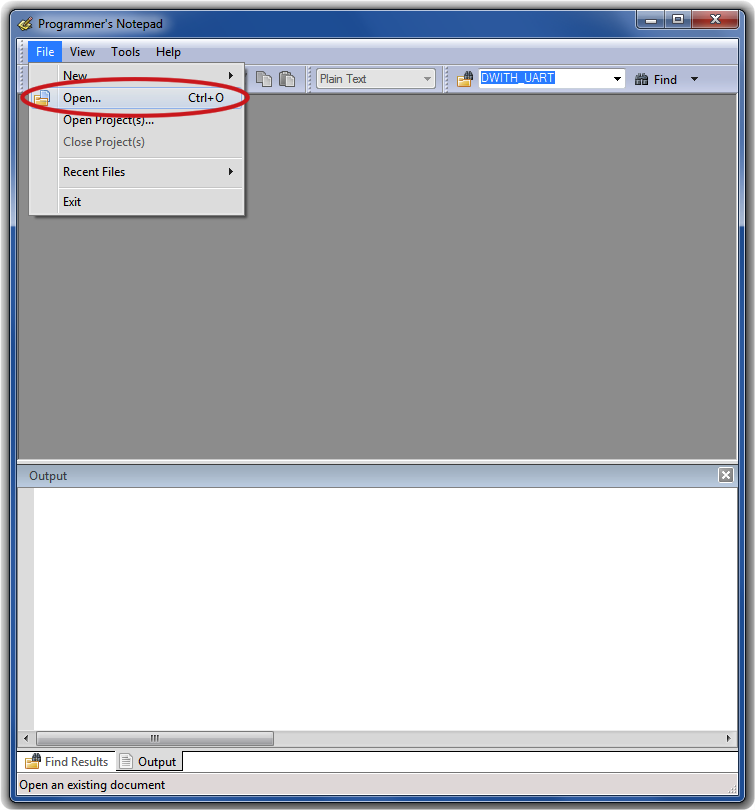
\includegraphics[width=.85\textwidth]{../PNG/Notepad_open.png}
    \caption{open Makefile}
  \end{subfigure}
  ~
  \begin{subfigure}[b]{.5\textwidth}
    \centering
    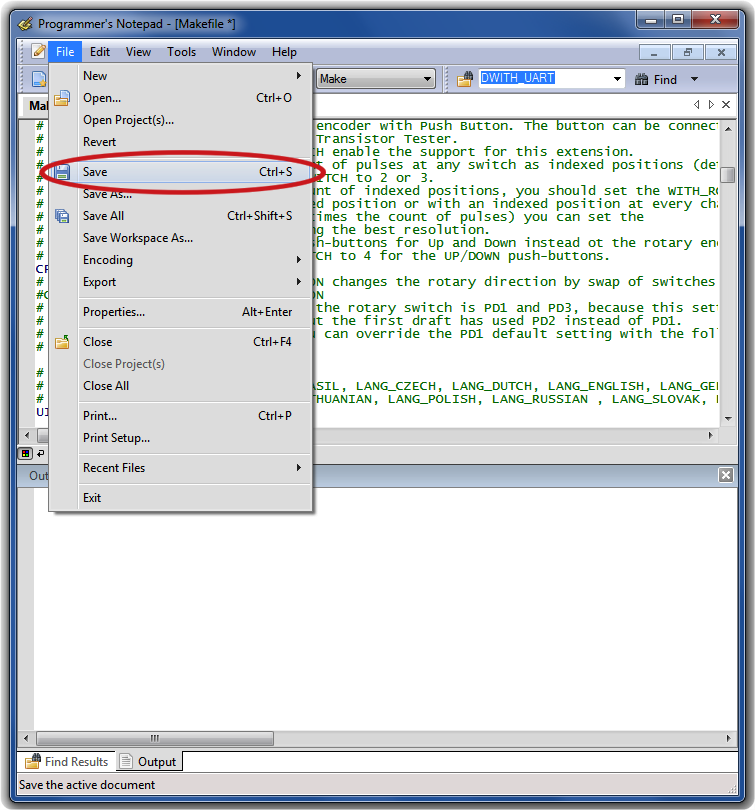
\includegraphics[width=.85\textwidth]{../PNG/Notepad_save.png}
    \caption{save Makefile}
  \end{subfigure}
  \caption{Using of the WinAVR user interface Programmer's Notepad}
  \label{fig:WinAVR1}
\end{figure}

The next figures~\ref{fig:WinAVR2} show the Tools menu of the Programmer's Notepad
for compiling the program (Make All) and for programming the ATmega (Program) with \lcmd{avrdude}.

\begin{figure}[H]
  \begin{subfigure}[b]{.5\textwidth}
    \centering
    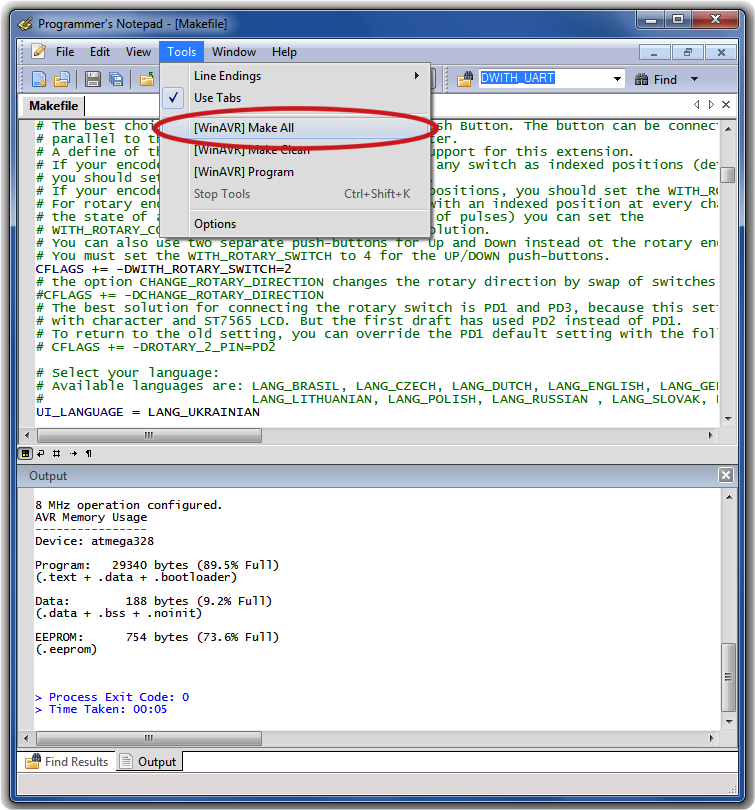
\includegraphics[width=.85\textwidth]{../PNG/Notepad_make.png}
    \caption{Build programming data (.hex/.eep)}
  \end{subfigure}
  ~
  \begin{subfigure}[b]{.5\textwidth}
    \centering
    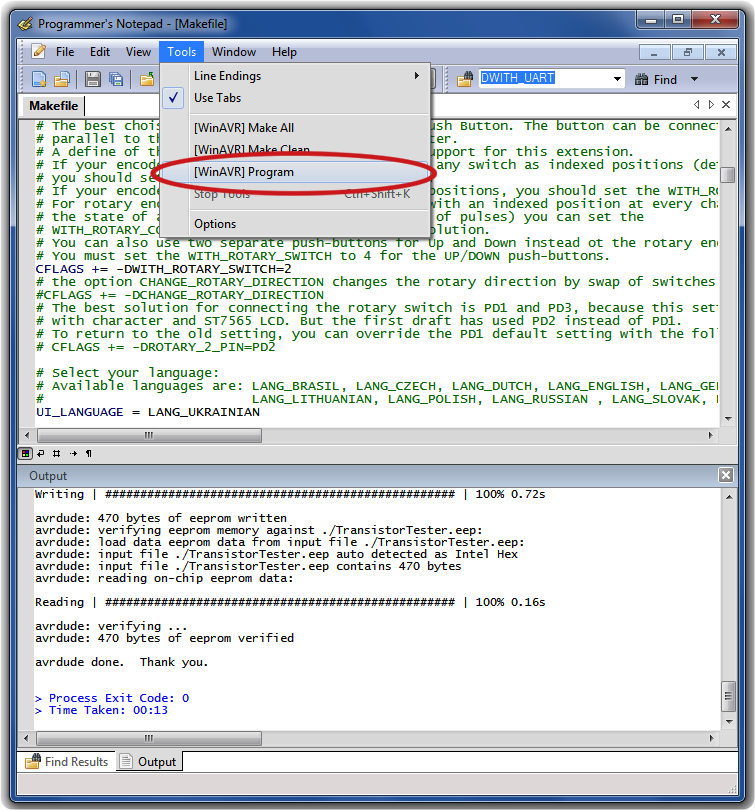
\includegraphics[width=.85\textwidth]{../PNG/Notepad_program.png}
    \caption{Programming the ATmega}
  \end{subfigure}
  \caption{Using of the WinAVR user interface Programmer's Notepad}
  \label{fig:WinAVR2}
\end{figure}



\section{Troubleshooting}
In most cases of problems you will miss the text output to the LCD-display.
At first you should check, if the LED was illuminated weak, if you release
the Test button. 
\begin{description} \setlength{\itemsep}{0em}

\item[Power does not switch on.]
If the LED is without light and the VCC power has correct
\(5V\) voltage during holding the Test button, the microcontroller does not switch the power
correctly. The microcontroller should hold the power by switching the
PD6 output to \(5V\), which is usually done as one of the first actions.
If you hold the Test key pressed, the power is switched on anyway.
So you can check the value of VCC power and additionally the voltage value
of the PD6 output, if you hold the key pressed.
If VCC voltage has correct value (\(5V\)), but PD6 voltage is
below \(4V\), your microcontroller does not start the program. In this case
you should check if the microcontroller flash has been loaded with proper data for your
installed type and if ATmega is correctly configured with the fuses.
If your ATmega put the PD6 output to \(5V\) and the power does not stay if you
release the Test key, it is more difficult to find the reason.
First you can shorten the LED and try again. If your Tester now starts,
your LED may be faulty or mounted with wrong polarity. If this is not
the reason, the current amplification factor of your T3 transistor (BC557C)
is insufficient. The current to the base of T3 is lower in the microcontroller
state as in the \inquotes{key pressed} state.

\item[Nothing is readable on the LCD display]
Check the voltage at the contrast pin at the LCD display (pin 3). Adjust to
correct value specified in the data sheet of your display and optimize by viewing.
If you have a high temperature display type, you must provide a negative contrast voltage
for operation. In this case you can use the ICL~7660 device for generating
a negative voltage from positive \(5V\).

The tester software can be configured for many different controller with different connection
types. You should check, if your software matches to your mounted display type.
If there is no output readable on the LCD and the background light is on,
you should disconnect the power and check all four data plus the two control signal connections.
If all connection are well, the only reason I see is a uncorrect timing of
control signals. This can be caused by a slower LCD controller than expected by
the software or the ATmega software runs at wrong clock speed. Please check for which
clock speed your programming data was compiled  and if the fuses of the
ATmega are correct set to that speed. You find the clock parameter in the corresponding
Makefile.
If the tester is build without the switch off electronic, you can test with
a LED connected to the test pins, if the program operates normally.
If the LED flickers, the program operates well. The missing text on the
LCD must be caused by wrong connection or timing.
For some graphical displays the contrast is changeable with a menu function.
If you have changed the contrast value, that nothing is readable at the screen,
you cannot handle the menu function any more. You can try to read the display
from a slanting look to the display, not from the front side.
In this case you can try to handle the menu function with this view.
Otherwise you can write the EEprom data new with a ISP programmer to reset the contrast value.


\item[Something but not all is readable on the LCD display]
Check if the .eep data are loaded to the EEprom memory of ATmega.
If all data are loaded correctly, you should check the clock speed of your
programming data (Makefile) and ATmega processor settings (fuses).

\item[Measurement is slow] and Capacitors are measured about 8 times too small
You run software compiled for \(8MHz\) clock at real clock speed of \(1MHz\).
Please set the fuses of the ATmega correctly.

\item[Measurement has strangely values]
Check if your programmer is still connected to the ISP-plug.
The ISP interface should be disconnected for measuring.
Very often the reason of wrong measurements is the use of software compiled with
the AUTOSCALE\_ADC option and with the option NO\_REF\_CAP, but the capacitor
at the AREF pin has still a value of \(100nF\).
Wrong assembly of components or remaining soft solder flux can disturb the 
measurements too. Please check with the selftest function of your TransistorTester software
if possible. For the details see Chapter~\ref{sec:selftest}.

Otherwise inspect your board visually and check the resistor values
with a ohmmeter. You can use the pins of the ATmega for this check, for example
to check the R1 you can measure between pin 23 and pin 14. Take a look at the
circuit diagram~\ref{fig:ttester} for details. There is no need to
remove the microcontroller, only battery or power supply should be removed before.

\item[The Tester switch off the power after 2 seconds display time] 
This condition exists, if the external Pull-Up resistor at the PD7 input
is missing or the key button is keep pressed.
The software switch off the internal Pull-Up resistors to prevent a influence
to the measurement results. Therefore a external Pull-Up resistor (27k) is required.

\item[Der Tester shows only Vext=xx.xV in row 2]
This problem exists, if the Pull-Up resistor at the PD7 input
is missing or the key button is keep pressed.
Additionally the software is configured without the serial output (without option WITH\_UART) and
without the internal Pull-Up resistors (with option PULLUP\_DISABLE).
You should install the Pull-Up resistor at pin PD7.


\end{description}
